%=============================================================================
%   About pentominos
%   Reporte de pentominos - Brief Summary
%   Servicio social - Laura Natalia Borbolla Palacios
%=============================================================================

\subsection{Pentominos}
% Hey, there! We are talking about pentominos. Basic structures and how
% Conway used them to find basic configurations in the elemental automata.
For more information, please consult \cite{language-and-automata-journal,
polyomino-life-wiki, rit-people, rpentomino-life-wiki, methuselah-life-wiki}.

A polyomino is a finite collection of orthogonally connected cells; or, in
another workds, a collection of equally-sized squares that form a connected
piece, meaning that each square can reach any other in it by going through
adjacent squares; the order of a polyomino is the number of squares used to
make it, so a fifth order polyomino (made of five squares), is called
pentomino. Both terms, polyomino and pentomino were first used by S. Golomb in
1953, in a talk to the Harvard Mathematics Club and a year later in an article.
There are twelve distinct pentominoes (see
Figure~\ref{fig:conway_pentominoes}) and two naming conventions, in
this paper the Conway convention (using letters \textit{O} through \textit{Z})
will be used; although the resemblance to the letters with this labeling scheme
seems a little more strained with the other scheme, specially when using the
\textit{O} instead of \textit{I}, it has the advantage that uses 12
consecutive letters; also, the Conway scheme tends to be used when discussing
topics related to cellular automata.

\begin{figure}[H]
	\centering
	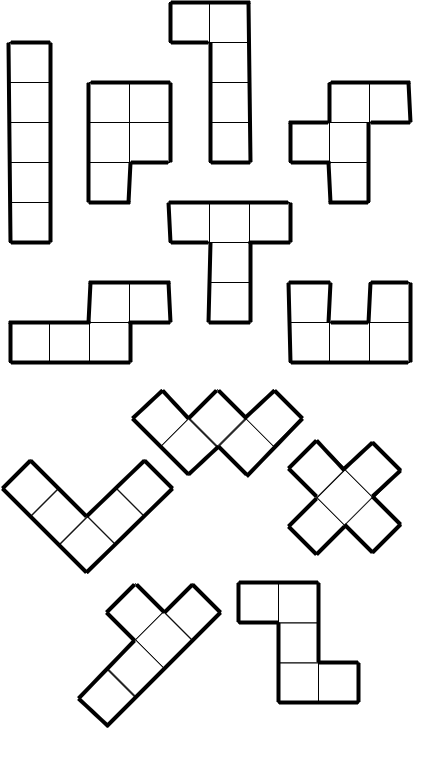
\includegraphics[scale=0.25]{diagrams/conway_pentominoes.PNG}
	\caption{Conway pentominoes from O through Z (left to right).}
  \label{fig:conway_pentominoes}
\end{figure}

Conway used polyominoes, specially pentominoes, in his initial investigations of
Life and other cellular automata: he tracked the histories of small polyominoes
as a way to explore the behaviour of different cellular automata when the
calculations had to be done by hand; the studies of the polyominoes led to
important discoveries in Life.

\subsubsection{R-Pentomino}
Among the other pentominoes, the \textbf{R-pentomino} outstands; mainly because
of two reasons:
	\begin{itemize}
		\item It is a methuselah\footnotemark, meaning is a pattern that takes a
			large number of generations to stabilize and, at some point during it's
			evolution, becomes much larger than it's initial configuration.
		\item The first glider ever observed is the glider that releases in the
		 	69th generation.
	\end{itemize}
Since all the others pentominoes stabilize in ten generations or less, this is,
by far, the most active pentomino: it takes 1103 generations and by then it's
population is of 116.

\footnotetext{
	M. Gardner defined methuselahs as patterns of less than ten cells that take
	more than fifty generations to stabilize\cite{ wheels-gardner}.}
